\documentclass{article}
%\usepackage[utf8]{inputenc}
\usepackage[top=0.9in, bottom=1in, left=1in, right=1in]{geometry}
\usepackage{comment}
\usepackage{amsthm}
\usepackage{amssymb}% http://ctan.org/pkg/amssymb
\usepackage{pifont}% http://ctan.org/pkg/pifont
\usepackage{xcolor}
\usepackage{multirow}
\usepackage{hhline}
\newcommand{\cmark}{\ding{51}}%
\newcommand{\xmark}{\ding{55}}%
\usepackage{amsmath}
\usepackage{algorithm}
%\usepackage{algorithmic}
\usepackage{algpseudocode}
\usepackage{graphicx}
\usepackage{caption}
\usepackage{subcaption}
%\usepackage{lscape} 
\usepackage{pdflscape}
\usepackage{rotating}
\usepackage{multirow}
\usepackage{hhline}
\usepackage{comment}
\usepackage{float}
%cmark xmark
\usepackage{pifont}
\usepackage{color}
\usepackage{longtable}
\usepackage{multicol}
\usepackage{setspace}
\usepackage{authblk}
\providecommand{\keywords}[1]{\textbf{\textit{Key words: }} #1}
\doublespacing


\usepackage[round, sort]{natbib}

\title{An Improved Genetic Algorithm for Multi-objective Dynamic Scheduling Optimization}
\author[1]{Kunlei Lian}
\author[1]{Chaoyong Zhang}
\author[1]{Liang Gao}
\author[1]{Chaoyang Zhang}
\affil[1]{State Key Laboratory of Digital Manufacturing Equipment and Technology, Huazhong University of Science and Technology, Wuhan, 430074}
\date{}

\begin{document}

\maketitle

\begin{abstract}
A CCA was developed and modified to solve the problem of minimal candidates set.
The minimal candidate set was a minimal hitting set.
The modified CCA improved performance in initialization, assimilation and rebirth of original CCA by introducing a third type of country, independent country, to the population of countries maintained by CCA by introducing a third type of country, independent country, to the population of countries maintained by CCA.
Implementation details of the proposed CCA and modified colonial competitive algorithm (MCCA) were elaborated using an illustrative example.
The performance of the algorithms was analyzed, and the results by the MCCA were compared with DMDSE-Tree algorithm.
When 90\% of the minimal hitting sets are obtained, the MCCA has better efficiency.
Finally, the experimental results of certain system verify the effectiveness of the algorithm, which proves that this method can be applied in solving the minimal hitting set of combinatorial optimization problems for selection of equipment effectively.
\end{abstract}


\keywords{Business planning; colonial competitive algorithm (CCA); minimal hitting set; equipment selection}

\doublespacing


\section{Introduction}
Assembly line is a widely used component in manufacturing enhancements, and various challenges emerge in its design and daily operations, among which the assembly line balancing problem (ALBP) exists as one of most significant ones.
It is noted that a small improvement towards ALBP can lead to significant efficiency enhancement and cost reduction \citep{salveson1};
On the other hand, ALBP is a classical NP-hard combinatorial optimization problem in which the complexity increases exponentially with the number of jobs and there yet exist polynomial-time algorithms to obtain optimal solutions in reasonable computation times \citep{kilincci2}.
Three solution strategies towards solving the ALBP can be found in the literature, namely, exact algorithms, heuristic algorithms and artificial intelligence algorithms.
Exact algorithms are able to find optimal solutions, but often require tremendous computation power and time.
Due to these limitations, they are mainly used to solve small-sized problems and can hardly be applied in real-world production systems \citep{scholl3, peeter4}.
Heuristic algorithms have received many attentions from the research community due to its implementation simplicity; however, they generally take long time to identify optimal solutions and also it is often hard to verify whether the solutions they found are optimal or not \citep{ponnambalam5}.
Artificial intelligence algorithms, including genetic algorithms, simulated annealing and tabu search, witness significant advancements in recent years and have been applied to solve the ALBP successfully \citep{azcan6, azcan7}.

Ant colony optimization (ACO) is an intelligent optimization algorithm proposed by Clolrni \citep{inproceedings8} in 1991 and has been applied to various combinatorial optimization problems.
\citet{bautista9} made the first attempt to solve a simple assembly line balancing problem using ant colony algorithms based on an ant system, but the optimization results were not optimal.
\citet{patrick10} obtained superior ACO performance on a number of benchmarking instances in solving a more complex assembly balancing problem that is characterized by mixed job types, stochastic processing times and parallel workstations.
\citet{bautista11} studied an assembly balancing problem with timing and spatial constraints and explored its solution method based on ant colony algorithms.

The aforementioned researches in solving assembly balancing problems using ACO suffer various performance issues when compared with other algorithms in the literature.
Some of them employ an oversimplified pheromone updating strategy that jeopardizes ACO's ability to converge to optimal solutions. 
Others use simple objective functions that often fail to correctly evaluate solution qualities, which results in inferior performance in identifying promising solutions.
To address these issues, we propose an adaptive ACO to solve the assembly line balancing problem.
It tries to avoid local optima by utilizing both external and historical information to adaptively adjust global pheromone evaporation factor in the process of ant path construction.
In addition, the algorithm incorporates balancing and smoothing factors in the objective function, which improves ACO's ability in identifying promising solutions.
Performance of the proposed algorithm is validated on benchmarking instances.

\section{Dynamic Scheduling Problem Description}
Static scheduling problems involve $n$ jobs to be processed on $m$ machines and the scheduling plan can be determined after the processing order is decided for every job on all the machines.
However, in real-world manufacturing systems, this processing order needs to be rescheduled whenever new orders arrive, machines break down or raw materials get delayed.

Dynamic scheduling views the job manufacturing as a dynamic process in which jobs become available for processing continuously, followed by machine processing and exiting the manufacturing system after their processes are finished.
Dynamic events refer to entities that trigger the rescheduling of existing jobs due to changes in scheduling environment, and they can be classified into four categories:
\begin{itemize}
	\item job-related events, these include stochastic arrivals of jobs, undetermined job processing times, changes in delivery date, dynamic priorities and orders.
	\item machine-related evenst, these include machine break-down, limited capacity, machine deadlock and conflicts in manufacturing capacity.
	\item process-related events, these include process delay, quality negation and output unstability.
	\item other events, these include absent operators, delayed arrival or unexpected flaws of raw materials, and dynamic processing routes.
\end{itemize}

In the classical job shop static scheduling problems, the release times $r_i$ of all jobs are assumed to be zero and the objective is to minmize the makespan $C_{max}$, which is defined as the maximum completion time of all jobs, $C_{max} = \text{min}\{\text{max} C_i, i = 1, \cdots n\}$ where $C_i$ is the completion time of job $J_i$.
In real-world dynamic manufacturing environments, however, jobs become available for process sequentially, meaning that their release times $r_i$ are different and unpredictable. 
Since a job can only be processed after it becomes available, in dynamic scheduling problems, the maximum completion time of all jobs is determined by the completion time of the latest-released job.
Therefore, dynamic scheduling problems generally use the mean flow time of all jobs as the objective function instead of the maximum completion time of all jobs.

This paper considers two performance metrics often seen in dynamic manufacturing environments: 1) minimization of mean flow time $\bar{F}$ where $\bar{F} = \text{min}(\frac{1}{n} \times \sum_{i = 1}^n C_i - r_i)$ and $r_i$ and $C_i$ are the release time and completion time of job $J_i$, respectively.
2) minimization of the weighted objective of maximum completion time $C_{max}$ and total tardiness. This weighted objective gives higher priority to urgent jobs which are required to finish by their due dates, and minimizes the completion times of remaining jobs.
For a scheduling problem with $n$ jobs and $m$ machines, the objective can be defined as follows:
\begin{align}
	\text{min}(\text{max}C_i + \alpha \times (\sum\text{max}(0, C_j - D_J))), \ (i \in S_{J_1}, j \in S_{J_2})
\end{align}
where $\alpha$ is the weighted penalty coefficient, $S_{J_1}$ is the job set that is being processed and $S_{J_2}$ is the newly inserted urgent job set, $C_i$ is the completion time for job $i \in S_{J_1}$, and $D_j$ is the delivery date for urgent job $j \in S_{J_2}$, and $C_j$ is the completion time.
\section{Rolling Scheduling Strategy}
Job scheduling in real-world manufacturing systems is not deterministic due to unpredictable events or random disturbances.
Raman \citep{raman19933} and Jian\citep{jian19972} apply the rolling horizon strategy to convert a nondeterministic scheduling problem into a series of dynamic but deterministic scheduling problems.
This is based on the successful industry applications of utilizing predictable control in continuous systems to replace optimal control, in which the scheduling process is divided into continuous static scheduling horizons and each one is solved sequentially.
This strategy is able to address the impact of nondeterministic factors in dynamic processing as well as incorporate system changes into scheduling plans.

Rolling horizon optimization is the key to rolling scheduling, during which completed jobs are first removed from the current scheduling horizon and new available jobs are then included, followed by rescheduling of updated jobs. 
This process is repeated until all jobs are finished processing.
The selection of rolling horizon and job selection strategy play key roles in the overall scheduling efficiency.

Applying rolling horizon into scheduling problem requires defining a rolling horizon which encompasses multiple job sets: finished job set, scheduled and processing job set, scheduled but not processing job set, available job set.
In every rolling scheduling step, finished job set is first removed from the current rolling horizon, and available job set is then added, followed by static scheduling optimization of this new job set.

The rescheduling cycle is defined as the time interval of two consecutive scheduling.
Normally, rescheduling times are evenly distributed, which does not consider the workload status of real-world manufacturing systems.
A more reasonable approach is to associate rescheduling frequency with manufacturing workload.
The number of jobs to be scheduled is limited by two factors: 1) it is preferred to select more jobs in the current scheduling horizon in order to improve machine utilization; 2) it is less desired to have too many jobs in the current horizon in order to reduce response times for urgent job insertions.
The decision is largely based on real-time circumstances.

There are three types of rolling horizon rescheduling: event-driven rescheduling, cycled rescheduling and hybrid rescheduling of the two.
Event-driven rescheduling refers to a rescheduling triggerred by the advent of system status-changing events, which may include delayed arrivals of raw materials, delayed processing and machine break-downs.
Cycled rescheduling refers to a rescheduling strategy controlled by pre-defined time intervals, which can be decided by planned deliveries, manufacturing workloads.
There two strategies are not able to incorporate future events and cycled rescheduling cannot tackled urgent events\citep{jian19972}.
The hybrid strategy is more responsive to real-world dynamic manufacturing environments and therefore more stable.
This paper employs this hybrid strategy by using cycled rescheduling as the general strategy and switching to event-driven rescheduling when urgent jobs emerge, including delayed raw materials arrive, machines break down, job delivery dates change and urgent jobs arrive.
\section{Dynamic Scheduling Strategy}
This paper proposes an improved genetic algorithm within the rolling horizon framework utilizing the hybrid cycled and event-driven rescheduling strategy.
The job rescheduling within a horizon is achived by the proposed genetic algorithm and the solution can be used for exection.
The following sections introduce the main components of the dynamic scheduling problems.

\subsection{Dynamic scheduling solution encoding scheme}
This paper uses a process-based encoding scheme in which all the processes of a job are indicated by the job number, and the $k$th occurance of the job indicates the $k$th process of the job.

\subsection{Dynamic scheduling solution decoding scheme} 
The scheduling solutino decoding scheme refers to the determination of the starting times of all process on all machines based on the current solution chromosome and process plans.
For a process $i$, given a starting time $t_i$ and processing time of $p_i$, its completion time can be computed as $(t_i + p_i)$.
The preceeding process of process $i$ is denoted by $JP[i]$ and the preceeding process of machine is $MP[i]$ if it exists.
In dynamic scheduling problems, the machining starting times of jobs that are being processed or un-processing, and not the first process, can be calculated as 
\begin{align}
	t_i = \text{max}(t_{JP[i]} + p_{JP[i]}, t_{MP[i]} + p_{MP[i]})
\end{align}
the starting times of the first process can be computed as
\begin{align}
	t_i = \text{max}(\text{max}(t_{JP[i]} + p_{JP[i]}), t_{MP[i]} + p_{MP[i]})
\end{align}

For available processes, the starting time $t_i$ of the first process can be computed by 
\begin{align}
	t_i = max(r_i, t_{MP[i]} + p_{MP[i00]})
\end{align}

This paper uses a decoding algorithm based on greedy insertion and can gurantee to produce a feasible schedule after solution decoding.

\subsection{Crossover and mutation operators}
There exist many crossver operators in the literature, including PPX\cite{cheng1999tutorial4}, SPX\citep{wang2001effective5}, POX\citep{zhang6}, among which POX is able to inherit promising characteristics of parent solutions and is depicted in figure \ref{fig:fig1}.

The mutation operator randomly selects a gene and inserts it into another position in order to produce a small solution perturbation.


\begin{figure}[h!]
	\begin{center}
		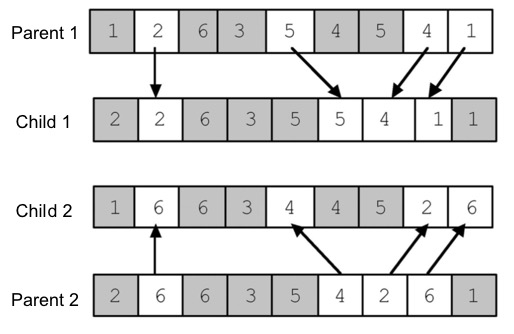
\includegraphics[width=0.6\linewidth]{sections/figure1.jpg}
		\caption{POX crossover operator based on job sequence encoding}
		\label{fig:fig1}
	\end{center}
\end{figure}

\subsection{Selection operartor}
Selection operator decides whether an individual enters the next generation based on its fitness value, which is defined as the objective function.
The selection operator in genetic algorithm uses both strategies of elite model and tournament selection.
The former identifies the best 1\% individuals in the current generation and allows them entering into the next generation directly without crossover.
Tournament selection works by randomly selecting two individuals from the current generation and then chooses the one with better fitness value if a random number $r \in (0,1)$ is smaller than a predefined value $k$ which is set as 0.8. 
Note that the chosen one will be allowed to be selected again in the next iteration of tournament selection.



\subsection{Improved genetic algorithm design}
Traditional genetic algorithm does not perform well in solving scheduling problems due to the acceptance of new offsprings created though the crossover operator, even if their fitness values are worse than that of their parent solutions, during which process good solutions are lost and damaged.
This paper proposes an improved genetic algorithm utilizing a new offspring solution creation strategy.
In this strategy, 2$n$ offspring solutions are created from $n$ iterations of crossover operators applied on two parent solutions, the two best offspring solutions are chosen as the final offspring solutions to enter the next iteration.
Computational results show that the improved algorithm performs superior than traditional genetic algorithm in both convergence rate and solution quality.
For example, the optimal solution with objective value of 930 is obtained using the improved genetic algorithm in solving the famous benchmark instance FT10.
The algorithmic workflow is as follows:
\begin{enumerate}
	\item randomly create $P$ chromosome individual solutions and compute their corresponding objective values.
	\item output the optimal solution if the stopping criteria is met; go to the next stop otherwise.
	\item select the offspring solutions for the next generation according to the selection operator.
	\item (1) apply crossover operator with probability $P_c$ on parent solution $n$ times to create 2$n$ offspring solutions, from which two best solutions are selected as the final offspring solutions; (2) apply mutation probability $P_m$ on offspring solutions to create mutated offsprings.
	\item create new population and return to step 2.
\end{enumerate}

\section{Experiments}
In this paper, we randomly generate 50 arrays of size 10 with values no greater than 20.
All the arrays are sorted non-decreasingly and all the equal numbers are set to 0.
The 50 arrays are then put into five groups: 1) the first group encompasses arrays 1 $\sim$ 10; 2) the second group encompasses arrays 1 $\sim$ 20; 3) the third group encompasses arrays 1 $\sim$ 30; 4) the first group encompasses arrays 1 $\sim$ 40; 5) the first group encompasses arrays 1 $\sim$ 50;
These generated instances are solved independently using the MCCA and the minimal hitting set algorithm based on dynamic maximum degree (DMDSE-Tree) \citep{c7zhang}.
For each group, the minimal hitting set and average computation times from five runs are recorded to make comparisons.

The experiments are run on a Windows XP computer with Intel Pentium G630 2.70 GHz CPU and 2GB memory.
All the algorithms are implemented using Visual C++ 6.0.
The parameters of MCCA are set as follows: $N_{pop} = 100$, $N_{imp} = 7$, $N_{ind} = 5$, the maximum number of iterations $N_{max} = 100$, the weight is set as $0.2, 0.3, \cdots, 0.8$ and $\alpha = 0.8$.
The minimal hitting set and computational time comparisons between MCCA and DMDSE-Tree are given table \ref{tab:tab1} and table \ref{tab:tab2}, respectively.


\begin{table}[h!]
	\begin{center}
		\caption{Computational results using DMDSE-Tree}
		\label{tab:tab1}
		\begin{tabular}{ccccccccc}
			\hline
			\multirow{2}{*}{group} & \multirow{2}{*}{size} & \multirow{2}{*}{No. MHS} & \multicolumn{6}{c}{computation time (s)} \\
			\cline{4-9}
			& & & 1 & 2 & 3 & 4 &5 & average time \\
			\hline 
			1 & 10 & 348  & 6.468  & 7.297  & 7.531  & 8.031  & 6.812  & 7.2287 \\
			2 & 20 & 861  & 21.932 & 21.671 & 22.734 & 20.750 & 22.172 & 21.8514 \\
			3 & 30 & 2426 & 43.343 & 43.109 & 43.297 & 43.688 & 44.250 & 43.5374 \\
			4 & 40 & 1618 & 61.516 & 59.562 & 59.953 & 58.828 & 58.921 & 59.7560 \\
			5 & 50 & 3165 & 89.797 & 88.406 & 88.562 & 87.281 & 87.187 & 88.2466 \\
			\hline
		\end{tabular}
	\end{center}
\end{table}



\begin{table}[h!]
	\begin{center}
		\caption{Computational results using modified CCA}
		\label{tab:tab2}
		\begin{tabular}{ccccccccc}
			\hline
			\multirow{2}{*}{group} & \multirow{2}{*}{size} & \multirow{2}{*}{No. MHS} & \multicolumn{6}{c}{computation time (s)} \\
			\cline{4-9}
			& & & 1 & 2 & 3 & 4 &5 & average time \\
			\hline 
			1 & 10 & 322  &  4.312 & 4.297   &  4.625 & 4.469  & 5.672   & 4.6570   \\
			2 & 20 & 766  & 15.219 &16.110   & 16.078 & 16.156 & 16.032  & 15.9190  \\
			3 & 30 & 1489 & 29.656 & 29.875  & 31.234 & 30.453 & 30.906  & 30.4248  \\
			4 & 40 & 2017 & 43.140 &  43.078 & 42.907 & 43.938 &  43.826 & 43.3778  \\
			5 & 50 & 2909 & 62.656 &  66.219 & 63.016 & 64.762 & 62.318  & 63.9942  \\
			\hline
		\end{tabular}
	\end{center}
\end{table}


The experiments are run five times and the average computation times and minimal hitting sets are obtained.
Table \ref{tab:tab3} shows the comparisons between computation time percentage and number of minimal hitting sets.

\begin{table}[h!]
	\begin{center}
		\caption{Comparison results}
		\label{tab:tab3}
		\begin{tabular}{cccccc}
			\hline
			& 1 & 2 & 3 &4 & 5 \\
			\hline
			MCCA time (s)        & 4.6750 & 15.9170 & 30.4248 & 43.3778 & 63.9942 \\
			DMDSE-Tree time (s)  & 7.2278 & 21.8514 & 43.5374 & 59.7560 & 88.2466 \\
			time percentage (\%) & 64.48  & 72.84   & 69.88   & 72.59   &  72.52  \\
			MCCA no. MHS         & 322    &  766    &  1489   & 2017    & 2909  \\
			DMDSE-Tree no.MHS    & 348    & 861     & 1618    & 2426    & 3165 \\
			\hline
		\end{tabular}
	\end{center}
\end{table}


It can be seen from table \ref{tab:tab3} that MCCA is able to solve 90\% of instances with about 70\% of computational times when compared to DMDSE-Tree, which shows the superior performance of MCCA in solving minimal hitting set problems.
In addition, MCCA shows better robustness in solving problems with various scales.
\section{Conclusions}
This paper proposes an adaptive ACO algorithm for the assembly line balancing problem.
It encompasses the following characteristics: comprehensive considerations of three rules of utilization, exploration and random search to construct feasible assignment plans; comprehensive considerations of assembly line balancing rate as well as smoothing factor to evaluate balancing performance to increase differentiation capability of different solutions; adaptive modifications of global pheromone evaporation factor in the construction phase to help the algorithm jump out of local optima and improve its global search capability. 
Computational results validate the superior performance of the proposed algorithm.

This paper only considers single deterministic assembly balancing problem and the proposed algorithm can be used to solve more complex assembly balancing problems, like dynamic problem, stochastic problem, multi-objective problem and multi-model assembly line balancing problems.

\bibliographystyle{plainnat}

\bibliography{biblio}



\end{document}
